\documentclass{report}

\begin{document}
\chapter{Логическое проектирование реляционной модели базы данных}

\section{Нормализация отношений}

Выполнять процедуру нормализации будем над реляционной моделью 
данных, построенной один в один из ER-модели. 

На данный момент 
каждое отношение имеет следующие свойства:
\begin{itemize}
    \item в отношении нет атрибутов с одинаковым смыслом
    \item у отношения есть ключ
    \item все неключевые атрибуты функционально зависят от ключа целиком, но не от его части
    \item неключевые атрибуты нетранзитивно функционально зависят от ключей
\end{itemize} 
Чтобы получить 1НФ необходимо избавиться от неатомарных атрибутов. 
Абонент имеет неатомарный атрибут ФИО. Разделим его на три атрибута - 
фамилия, имя, отчество. Теперь все отношения в 1НФ.

Все неключевые атрибуты функционально зависят от ключа целиком и отношения
находятся в 1НФ, следовательно отношения находятся во 2 НФ. Далее, неключевые 
атрибуты нетранзитивно функционально зависят от ключей и отношения находятся
во 2НФ, следовательно отношения находятся в 3 НФ.

\section{Реляционная схема}

Все ссылочные (целевые) отношения имеют сурогатный ключ, который
нам незачем изменять. Поэтому для обеспечения ссылочной целостности
при удалении будем использовать политику каскадного удаления, 
а при обновлении - ничего не делать.

Кроме того, нам понадобится тип конечного устройства (телефона) - перечисление 
device\_type = (``Common'', ``Parallel'', ``Paired''). 
\newpage
\begin{longtblr}[caption={Реляционная схема базы данных}, theme = TC,]{
        colspec={|X[3]|X[3]|X[3]|X[1]|X[4]|}, row{1} = {c}, hlines,
    }
    Отношение & Атрибут & Тип & Not null & Ограничения \\
    \SetCell[r=4]{c} ATS & ats\_id & serial & + & PK \\ 
    & ats\_owner & text & - & \\
    & first\_phone\_no & int & + & $(0, 1'000'000'000)$ \\
    & last\_phone\_no & int & + & $(1, 1'000'000'000)$, $last>first$ \\ 
    \SetCell[r=1]{c} City ATS & ats\_id & int & + & PK-FK \\
    \SetCell[r=1]{c} Department ATS & ats\_id & int & + & PK-FK \\
    \SetCell[r=1]{c} Institution ATS & ats\_id & int & + & PK-FK \\ 
    \SetCell[r=3]{c} Phone & phone\_id & serial & + & PK \\
    & ats\_id & int & + & FK \\ 
    & address\_id & int & + & FK \\ 
    \SetCell[r=1]{c} Payphone & phone\_id & int & + & PK-FK \\
    \SetCell[r=3]{c} Phone number & phone\_id & int & + & PK-FK \\ 
    & apartment & int & - & $>0$ \\ 
    & phone\_no & int & + & $(0, 1'000'000'000)$ \\
    \SetCell[r=8]{c} Subsriber (Абонент) & subsriber\_id & serial & + & PK \\ 
    & first\_name & text & + & \\
    & last\_name & text & + & \\
    & surname & text & - & \\
    & sex & char (1) & - & `m' или `f' \\
    & age & smallint & - & $[14, 130]$ \\ 
    & benefit & numeric (3, 2) & + & $[0, 1.00], default=0$ \\ 
    & debt & numeric (10, 2) & + & $\geq 0, default=0$ \\ 
    \SetCell[r=4]{c} Subsription (Абонемент) & subsription\_id & serial & + & PK \\ 
    & phone\_id & int & + & FK \\
    & subsriber\_id & int & + & FK \\
    & phone\_type & device\_type & + & $default=$ Common \\ 
    \SetCell[r=3]{c} Service (Услуга) & service\_id & serial & + & PK \\ 
    & service\_name & text & + & \\
    & service\_cost & numeric (10, 2) & + & $\geq 0, default=0$ \\
    \SetCell[r=3]{c} Service Connection & subsription\_id & int & + & PK-FK \\ 
    & service\_id & int & + & PK-FK \\
    & payment\_date & date & + & $default=$ current date \\
    \SetCell[r=4]{c} Call log & initiator & int & + & PK-FK \\ 
    & call\_time & timestamptz & + & PK \\
    & recipient & int & + & FK \\
    & duration & int & + & $>0, default=1$ \\
    \SetCell[r=2]{c} City & city\_id & serial & + & PK \\ 
    & city\_name & text & + & \\ 
    \SetCell[r=3]{c} District & district\_id & serial & + & PK \\ 
    & city\_id & int & + & FK \\ 
    & district\_name & text & + & \\ 
    \SetCell[r=3]{c} Street & street\_id & serial & + & PK \\ 
    & district\_id & int & + & FK \\ 
    & street\_name & text & + & \\ 
    \SetCell[r=3]{c} Address & address\_id & serial & + & PK \\ 
    & street\_id & int & + & FK \\ 
    & house\_no & int & + & $>0$ \\ 
\end{longtblr}

\begin{figure}[!ht]
    \begin{center}
    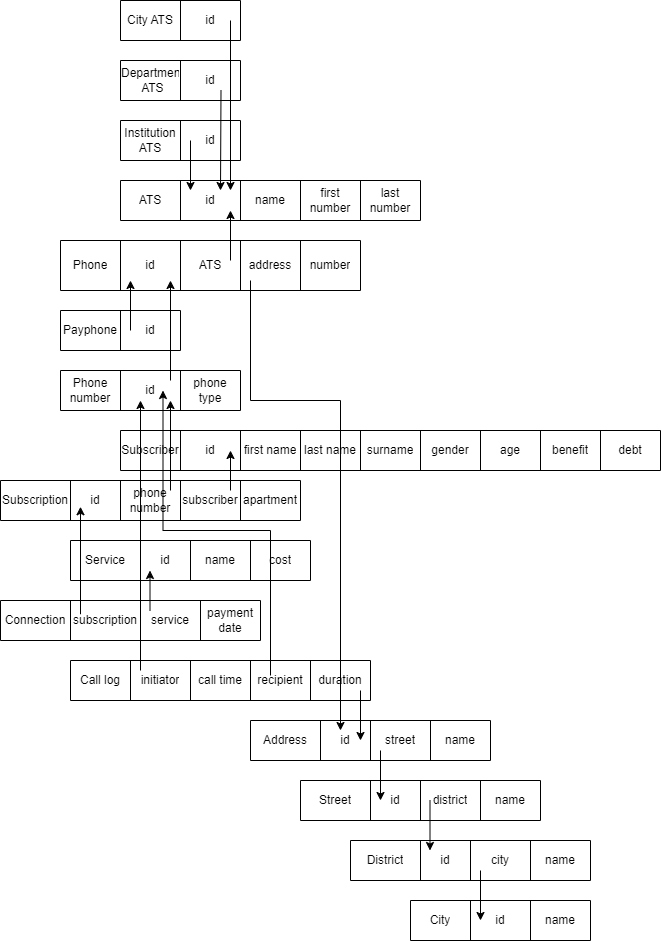
\includegraphics[height=0.9\textheight, keepaspectratio, width=\textwidth]{resources/vertical.png}
    \caption{Вертикальная диаграмма}
    \end{center}
\end{figure}

\end{document}
